% Asset ID: FA22GameTheoryEnrichmentTikZ-002
% Source: Transcript graphical method for 2 by 3 or 3 by 2 games
% Core CCEA status: Optional enrichment only
\documentclass[tikz,border=8pt]{standalone}
\usepackage{amsmath}
\usetikzlibrary{arrows.meta}
\definecolor{Canvas}{HTML}{FAF9F6}\definecolor{Ivory}{HTML}{FFFFF0}\definecolor{LineGrey}{HTML}{E5E5EA}\definecolor{AccentGold}{HTML}{C5A059}\definecolor{DeepGold}{HTML}{D4AF37}\definecolor{SoftPink}{HTML}{FBEFEF}\definecolor{MathText}{HTML}{2C2C2E}
\begin{document}
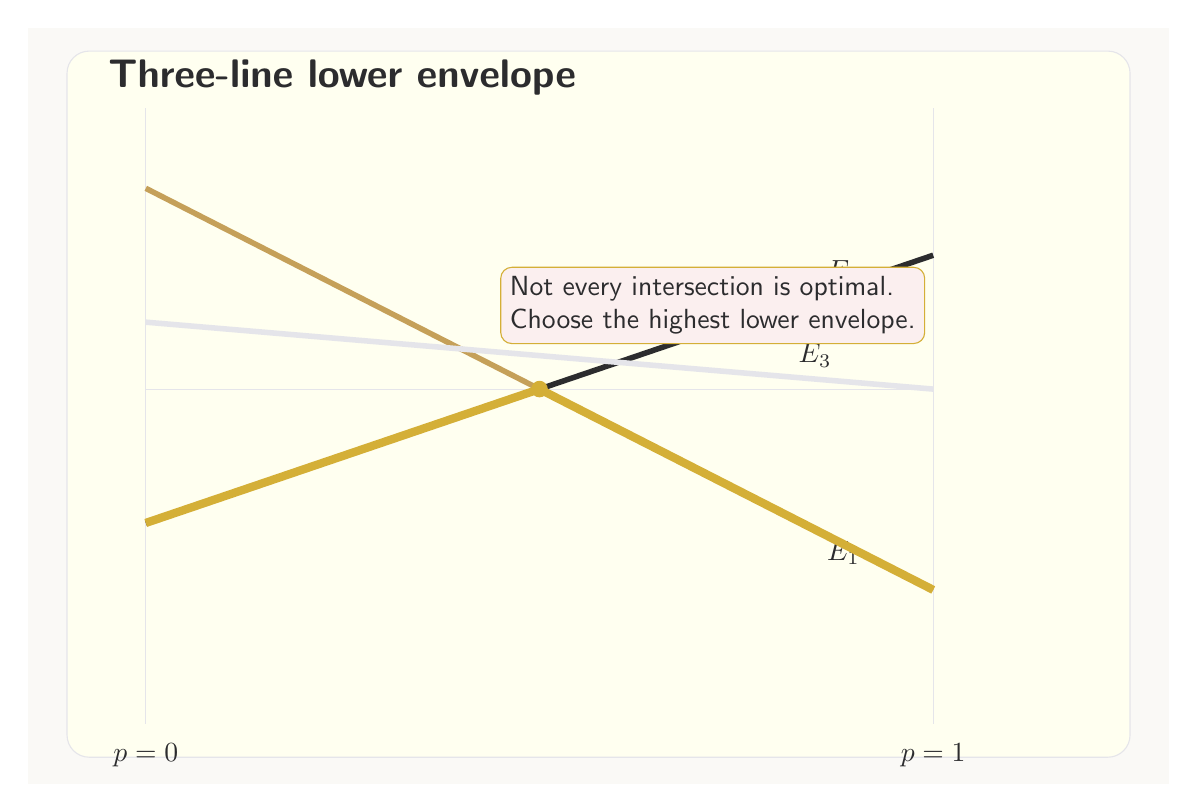
\begin{tikzpicture}[x=10cm,y=.85cm,>=Latex,every node/.style={font=\sffamily,text=MathText}]
\fill[Canvas] (-.15,-5.9) rectangle (1.3,5.4); \draw[LineGrey,fill=Ivory,rounded corners=8pt] (-.1,-5.5) rectangle (1.25,5.05);
\node[anchor=west,font=\sffamily\bfseries\Large] at (-.06,4.65){Three-line lower envelope};
\draw[LineGrey] (0,-5)--(0,4.2); \draw[LineGrey] (1,-5)--(1,4.2); \draw[LineGrey] (0,0)--(1,0);
\draw[AccentGold,line width=2pt] (0,3)--(1,-3) node[pos=.85,below right]{\(E_1\)}; \draw[MathText,line width=2pt] (0,-2)--(1,2) node[pos=.85,above right]{\(E_2\)}; \draw[LineGrey,line width=2pt] (0,1)--(1,0) node[pos=.85,above]{\(E_3\)};
\coordinate (I) at (.5,0); \draw[DeepGold,line width=3pt] (0,-2)--(I)--(1,-3); \fill[DeepGold] (I) circle (3pt);
\node[draw=DeepGold,fill=SoftPink,rounded corners=4pt,align=left] at (.72,1.25){Not every intersection is optimal.\\Choose the highest lower envelope.};
\node[anchor=north] at (0,-5.15){\(p=0\)}; \node[anchor=north] at (1,-5.15){\(p=1\)};
\end{tikzpicture}
\end{document}
